It all started when a renowned owl wearing a hat and monocle arrived.

``It's a pleasure to welcome you to the Grand Hotel Infinita,'' said Henrietta. ``A place where the longing quest is left behind, where you may rest and ease your weary mind.''
%``A place where the longing quest is left behind, where you may rest and leave the whirlpool of wild dreams behind.''

The owl replied with a peculiar request, ``Thank you, my dear. I would like a room on the first floor, for I am terribly afraid of heights.''

``The rooms on the first floor are completely full,'' Henrietta sighed. It was a common problem, as guests usually weren't fond of taking the stairs. But, trying to be as friendly and caring as possible, she added, ``But don't you worry!''

To accommodate this eminent guest, she called the distinguished walrus and, in the most delicate way, asked him to move from Room 1 on the first floor to Room 1 on the second floor. The walrus promptly agreed.

\vfill
\begin{center}
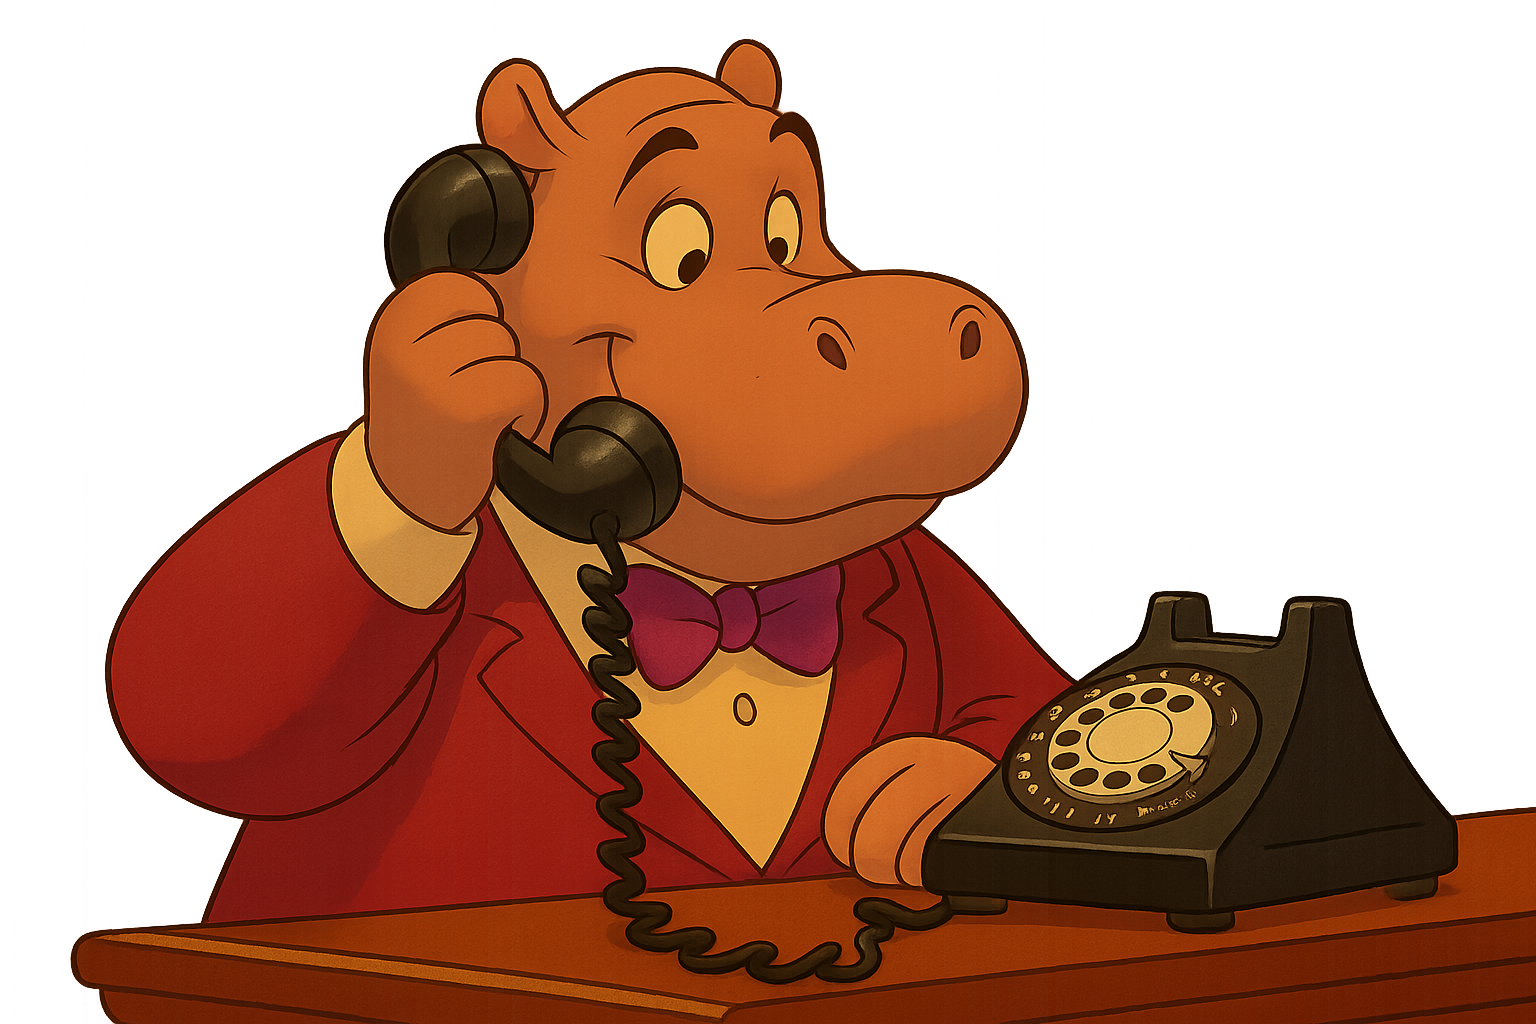
\includegraphics[width=0.5\textwidth]{images/telephone.png}
\end{center}

\clearpage
\includepdf[pages={1},
            pagecommand={\thispagestyle{fancy}}, % Apply your custom 'fancy' style
            fitpaper=true,
            noautoscale
           ]{elevator.pdf}

%To accommodate this eminent guest, she called the distinguished walrus and, in the most delicate way, asked him to move from Room 1 on the first floor to Room 1 on the second floor. The walrus promptly agreed. 
Bernard rapidly took the walrus's belongings and moved them up to the next floor using the small freight elevator.

``Bernard will help you to your new room at once!'' Henrietta added.

The owl was delighted to take the newly vacant room on the first floor, and Bernard quickly brought his luggage in.

A few minutes later, a graceful giraffe in a scarf and long socks appeared. With a dazzling look in her eyes, she entered, observing every detail of the grand hotel, and with her head held high, she almost hit it on the central chandelier. Bernard, seeing Henrietta getting ready to move the owl, suggested, ``Let's move the guest in Room 2 instead! The owl just settled in, and he's afraid of heights.'' Henrietta agreed. The giraffe, looking grateful, said, ``That is so kind of you! I won't have to struggle up and down the infinite stairs!'' Bernard swiftly took her belongings, and she was happily settled into her new room.

\vfill
\begin{center}
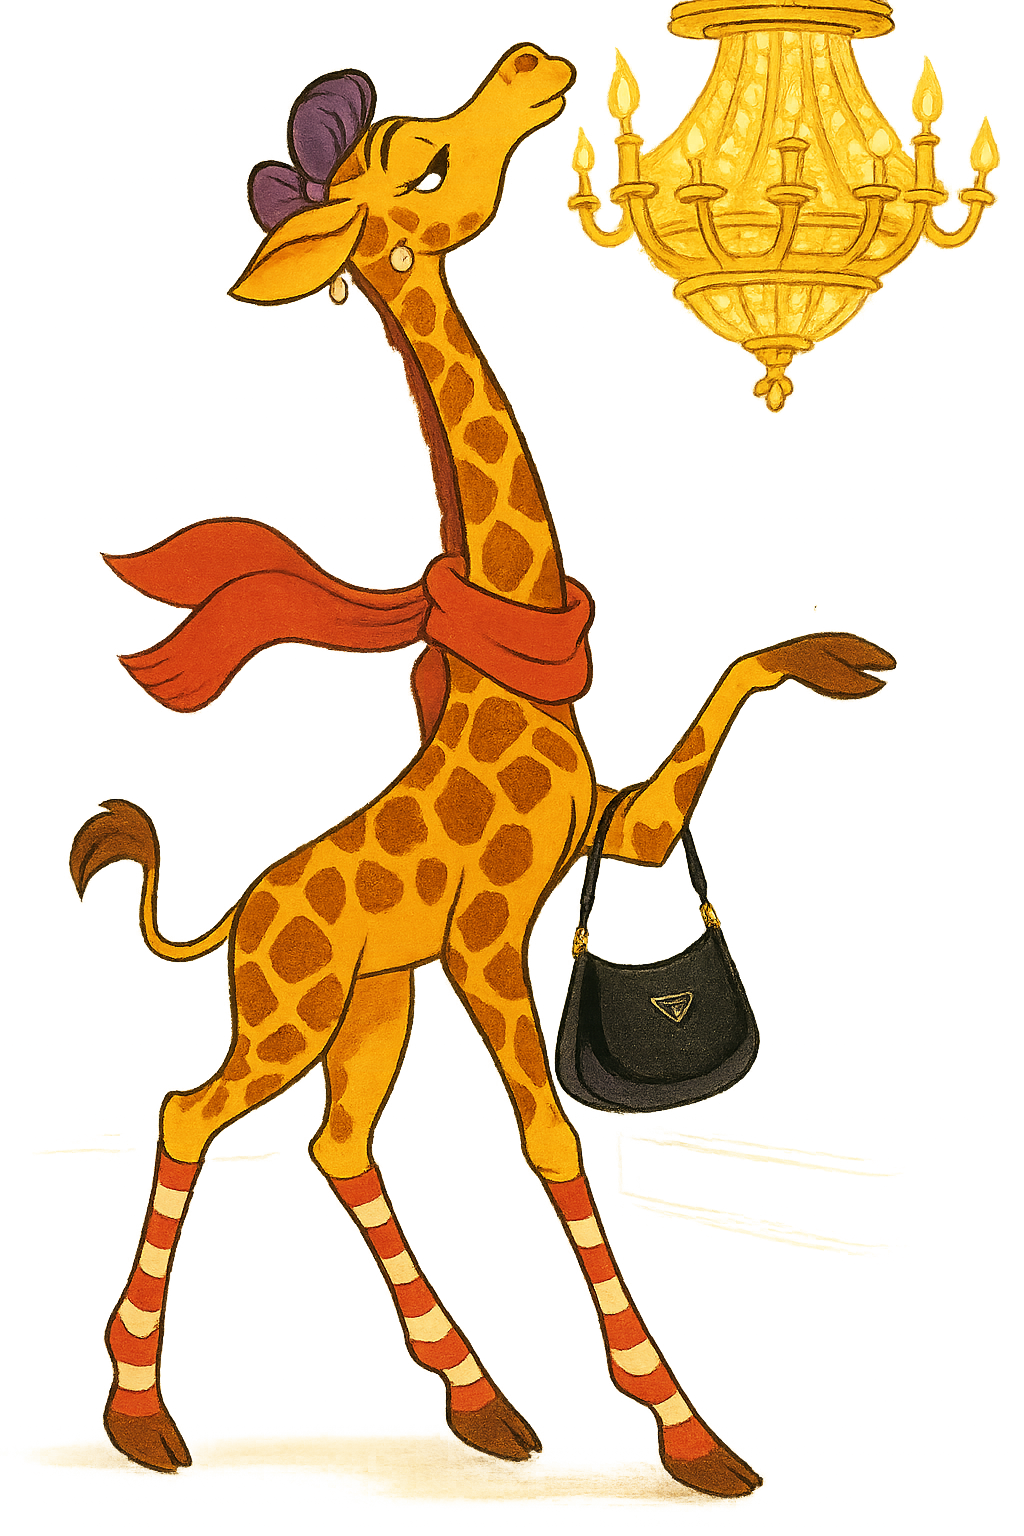
\includegraphics[width=0.45\textwidth]{images/giraffe.png}
\end{center}

\clearpage
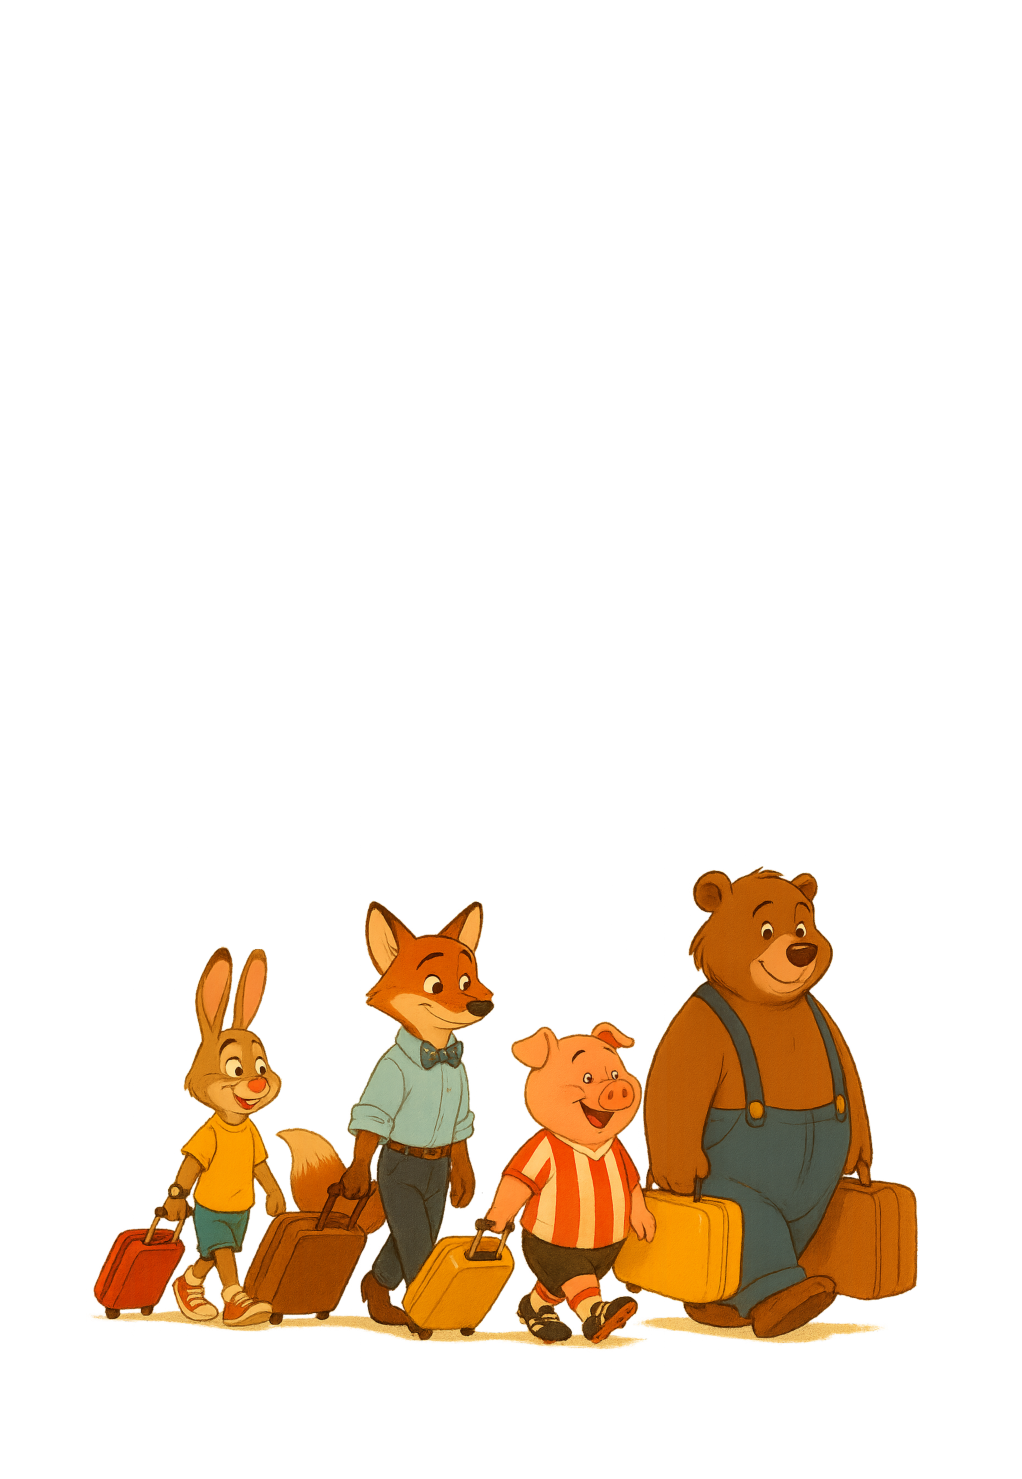
\includepdf[pages={1},
            pagecommand={\thispagestyle{fancy}}, % Apply your custom 'fancy' style
            fitpaper=true,
            noautoscale
           ]{checkinanimals.pdf}

Throughout the day, more and more animal guests arrived: a rabbit with a wristwatch, a fox with a bow tie, a pig with football boots, and a bear with suspenders. Each time, Bernard and Henrietta repeated their clever system, moving the next guest from the first floor to the second, always to the same numbered room. It was an ingenious solution to a peculiar problem. By the end of the day, they had received a total of 54,907 new guests, and it seemed like everyone was well accommodated... but it was just the start of a chaotic evening.
